%%% Local Variables:
%%% mode: latex
%%% TeX-master: t
%%% End:
% --------------------------------------------------------------
% This is all preamble stuff that you don't have to worry about.
% Head down to where it says "Start here"
% --------------------------------------------------------------

\documentclass[12pt]{article}

\usepackage[margin=1in]{geometry}
\usepackage{amsmath,amsthm,amssymb}
\usepackage{graphicx}

\newcommand{\N}{\mathbb{N}}
\newcommand{\Z}{\mathbb{Z}}

\newenvironment{theorem}[2][Theorem]{\begin{trivlist}
\item[\hskip \labelsep {\bfseries #1}\hskip \labelsep {\bfseries #2.}]}{\end{trivlist}}
\newenvironment{lemma}[2][Lemma]{\begin{trivlist}
\item[\hskip \labelsep {\bfseries #1}\hskip \labelsep {\bfseries #2.}]}{\end{trivlist}}
\newenvironment{exercise}[2][Exercise]{\begin{trivlist}
\item[\hskip \labelsep {\bfseries #1}\hskip \labelsep {\bfseries #2.}]}{\end{trivlist}}
\newenvironment{reflection}[2][Reflection]{\begin{trivlist}
\item[\hskip \labelsep {\bfseries #1}\hskip \labelsep {\bfseries #2.}]}{\end{trivlist}}
\newenvironment{proposition}[2][Proposition]{\begin{trivlist}
\item[\hskip \labelsep {\bfseries #1}\hskip \labelsep {\bfseries #2.}]}{\end{trivlist}}
\newenvironment{corollary}[2][Corollary]{\begin{trivlist}
\item[\hskip \labelsep {\bfseries #1}\hskip \labelsep {\bfseries #2.}]}{\end{trivlist}}

\begin{document}

% --------------------------------------------------------------
%                         Start here
% --------------------------------------------------------------

\newcommand{\ijk}{(i, j, k)}

\title{CS5214 Design of Optimizing Compilers }%replace X with the appropriate number
\author{Professor Weng-Fai Wong\\ %replace with your name
Assignment One} %if necessary, replace with your course title

\maketitle

\abstract{
This is my solutions for assignment three problem set.
This is the answer presented by Pan An. My student number is
A0134556A.
}
% --------------------------------------------------------------
%     You don't have to mess with anything below this line.
% --------------------------------------------------------------





\section{Loop Analysis}
The flow dependency of the given loop psudo-code concerns only
variable list $X$. Here we denote the only value assignment in the
loop as
$$X[\vec{f}\ijk] = X[\vec{g}\ijk]$$

\subsection{Formulation}
So in this case if we need to take care of the formulation there are
three equations that we need to satisfy:
\begin{equation}
\begin{aligned}
3j_s + k_s &= & 2i_t +4k_t\\
i_s + 2j_s + k_s &= & 5j_t + 7k_t\\
2j_s + 3k_s &= & 3i_t + 5j_t\\
\end{aligned}
\end{equation}

And $i, j, k$ subject to:

\begin{equation}
\begin{aligned}
0 < & ~i_s, i_t< 11\\
0 < & ~j_s, j_t< 51\\
0 < & ~k_s, k_t< 21
\end{aligned}
\end{equation}

%
%
%
So here I'm gonna go with formulating the problem with distance
vector.
The problem defined can be expressed in matrix form: $$\pmb{A\cdot X < b }$$
 where:
%%%%%%%%%%% problems here!
\begin{equation}
%\left[ \begin{array}{c} x_s \\ x_t \end{array} \right]
%= \begin{bmatrix} A & B \\ C & D \end{bmatrix} \times
%\left[ \begin{array}{c} y_s \\ y_t \end{array} \right]
 \pmb{A} =\begin{bmatrix}
 0 & 1  & 0  \\
 3 & 2  & 2  \\
 1 & 1 & 3 \\
-2 & 0 & -3 \\
0 & -5 & -5 \\
-4 & -7 & 0 \\

 \end{bmatrix}
\end{equation}
Which has to satisfy:

\begin{equation}
  [i_s, j_s, k_s, i_t, j_t, k_t] \begin{bmatrix}
 0 & 1  & 0  \\
 3 & 2  & 2  \\
 1 & 1 & 3 \\
-2 & 0 & -3 \\
0 & -5 & -5 \\
-4 & -7 & 0 \\

 \end{bmatrix}
= [0, 0, 0]
\end{equation}


And after Echelon Reduction we have(proof reading has been done with a
lot of A4 papers):
\begin{equation}
  \pmb{E} = \begin{Bmatrix}
    1 & 0 & 0 \\
0 & 1 & 0 \\
0 & 0 & 1 \\
0 & 0 & 0 \\
0 & 0 & 0 \\
0 & 0 & 0 \\
  \end{Bmatrix}
~~and~~ \pmb{U}
=
\begin{bmatrix}
  -\frac{4}{7} & \frac{3}{7} & -\frac{2}{7}  & 0 & 0  & 0 \\
 1 & 0 &  0 & 0 &  0 & 0 \\
 -\frac{1}{7} & -\frac{1}{7} & \frac{3}{7} & 0 & 0 & 0 \\
-\frac{11}{7}& -\frac{3}{7} & 0 & \frac{5}{7}  & 0 & 0 \\
\frac{30}{7} & -\frac{5}{7} & \frac{15}{7} & 0 & 1 & 0 \\
\frac{33}{7}& \frac{12}{7} & -\frac{8}{7} & 0 & 0 & 1 \\
\end{bmatrix}
\end{equation}

And in order to do finish the back substitution have to let
$\pmb{t\cdot E = 0}$. So we have:
$$t_1, t_2, t_3 = 0$$

which leads to the following:
\begin{equation}
  \begin{aligned}
    i_s &=  -\frac{11}{7}t_4+\frac{30}{7}t_5+\frac{33}{7}t_6\\
    j_s &=  \frac{3}{7}t_4-\frac{5}{7}t_5+\frac{13}{7}t_6\\
    k_s &=  \frac{5}{7}t_4+\frac{15}{7}t_5-\frac{8}{7} \\
    i_t, j_t, k_t &= t_4, t_5, t_6\\
  \end{aligned}
\end{equation}


\subsection{Fourier-Motzkin Elimination}
For the previous section we have the following:


\begin{equation}
  \begin{aligned}
    0 <&-\frac{11}{7}t_4+\frac{30}{7}t_5+\frac{33}{7}t_6 &\le 10 \\
    0 <& ~~~~~~\frac{3}{7}t_4-\frac{5}{7}t_5+\frac{12}{7}t_6 &\le 50 \\
0 <&~~~~~~ \frac{5}{7}t_4+\frac{15}{7}t_5-\frac{8}{7}t_6   &\le 20 \\
0 <& ~~~~~~~~~~~~~~~t_4 &\le 10 \\
0 <& ~~~~~~~~~~~~~~~t_5 &\le 50 \\
0 <& ~~~~~~~~~~~~~~~t_6 &\le 20 \\
  \end{aligned}
\end{equation}

%%%%%%%%%%%%%%% okay start from here %%%%%%%%%%%%%%%%%%%%%%%%

However, real solutions does not exist when I ran it with code. 

After the the  elimination we have:
\begin{equation}
  \begin{aligned}
    t_4 &\ge -\frac{122}{91}\\
    \frac{3}{5}t_4+t_5 &\ge \frac{1}{7}\\
    -\frac{11}{30}t_4+t_5&\ge -\frac{659}{30}\\
    -\frac{11}{25}t_4+t_5&\ge -\frac{3846}{175}\\
    \frac{11}{105}t_4+t_5&\ge \frac{41}{735}\\
    \frac{1}{3}t_4+t_5&\le 20\\
    \frac{3}{5}t_4+t_5&\le 32\\
    -\frac{3}{5}t_4+t_5&\le \frac{239}{5}\\
    -\frac{11}{25}t_4+t_5&\le \frac{269}{175}\\
    \frac{11}{105}t_4+t_5&\le \frac{148}{21}\\
    -\frac{5}{8}t_4-\frac{15}{8}t_5+t_6&\ge -\frac{35}{2}\\
    \frac{1}{4}t_4-\frac{5}{12}t_5+t_6&\ge \frac{1}{12}\\
    -\frac{1}{3}t_4+\frac{10}{11}t_5+t_6&\ge \frac{1}{33}\\
    -\frac{1}{4}t_4+\frac{5}{12}t_5-t_6&\ge -\frac{175}{6}\\
    \frac{1}{3}t_4-\frac{10}{11}t_5-t_6&\ge -\frac{70}{33}\\
    \frac{5}{8}t_4+\frac{15}{8}t_5-t_6&\ge \frac{1}{8}\\
  \end{aligned}
\end{equation}

which is a lot of math. I generated it with C++, I did it with hands
and got it wrong many times then I finally gave up since it took too
much time. 


I used a package in Nodejs and it shows that there IS solutions for
this one. However I performed the calculation by hand at first and
unfortunately failed again and again since the math might get very
dirty after a couple of eliminations. Code is also attached to the tarball.

\subsection{Omega Test}
With the constraints listed in the previous section, we can do omega
test to check if there are integer solutions for the problem. Omega
test involves a couple steps. First  the previous inequalities can be
used to derived the following facts:
\begin{equation}
  \begin{aligned}
    140t_5&\ge 761\\
    55t_5&\le 399\\
    -77t_4+175t_5&\le 269\\
    -77t_4+175t_5&\ge -3846\\
    77t_4+735t_5&\le 5180\\
    77t_4+735t_5&\ge 41 \\
    t_4+15t_6&\ge 1\\
    -21t_4+49t_6&\ge -279\\
    t_4 + 15t_6&\le 310\\
    -21t_4+ 49t_6&\le 68
  \end{aligned}
\end{equation}
I hope I did not make any mistaking of the input here. I will be
switching to Org-Mode later. Even Emacs has pretty good tools for
literal stuff there will still be a lot of mistakes in those formulas
when you input by hand.

With one step further:
\begin{equation}
  \begin{aligned}
    5t_5& \le 399 \\
    140t_5& \ge 761\\
    14t_6&\le 253\\
    182t_6&\ge -129\\
  \end{aligned}
\end{equation}

To avoid solving problems with meatball eyes, I followed the procedure
and found the $\aleph$ and $\beta$ for each of $t_5, t_6$. 

So for $t_5$, we have $\beta=761$, $b = 140$, $\alpha=399$, $a=5$. And
we have:
$$b\alpha - a\beta=140\times 399 - 5\times 761 = 52055$$
$$ba-a-b+1 = 556$$

Obviously there exists integer solution.

And for $t_6$:  $\beta=-129$, $b = 182$, $\alpha=253$, $a=14$. And:
$$b\alpha - a\beta = 47852$$
$$ba-a-b+1 = 2353$$

And the conclusion is that there is solution for this one. However I
thought there might not be solutions. 

\subsection{Brute Force}
The test with Python shows the following case was the solution for
dependency:
\begin{verbatim}
(10, 15, 9) (20, 22, 39)
    i=8,  j=3, k=1
(9, 17, 13) (32, 31, 40)
    i=10, j=2, k=3
\end{verbatim}

Well the first time I did not get any output since I wrote something
like this:

\begin{verbatim}
for i in range(1,11):
    for j in range(1,51):
        for k in range(1,21):
            key = 3*j+k, i+2*j+k, 2*j+3*k
            val = 2*i+4*k, 5*j+7*k, 3*i+5*j
            if key==val:
                print key, val
                print i,j,k
\end{verbatim}

This however, reminds me that after all the slides that I went
through, it becomes a little confusing when I really start to
code. The right solution should check if the value source is already
calculated before. And in this case, the right code should be:

\begin{verbatim}
x = {}
for i in range(1,11):
    for j in range(1,51):
        for k in range(1,21):
            key = 3*j+k, i+2*j+k, 2*j+3*k
            val = 2*i+4*k, 5*j+7*k, 3*i+5*j
            if val in x:
                print key, val
                print i,j,k
            x[key] = val
\end{verbatim}
And that's how I solved the problem.
\section{Loop Tiling}

Considering that in this problem X and Y has exactly the same size. There is no need to take into consideration
the utilization of loop interchange.

Anyway, the idea of loop tiling is to increase cache. 
Consider the given case:
\begin{verbatim}
for (int i = 0; i < n; ++i) {
    for (int j = 0; j < n; ++j) {
        X[i, j] = Y[j, i];
    }
}

\end{verbatim}
This however, will result in loading the data in X and Y 
unnecessary number of times. The program will miss every access to one
of the array and every step of $C$ on the other, where $C$ is the size
of the cache. And the total cache miss would be: $$N^2+\frac{N^2}{C}$$

And in this case it's $N^2+\frac{N^2}{8}$. 

Loop tiling code is shown as below(notice that both X and Y are
$N\times N$ matrix):
\begin{verbatim}

for(ii=0; ii<N; ii+=block_size)
    for(jj=0; jj<N; jj+=block_size)
        for(i=ii; i<min(ii+block_size); i++)
            for(j=jj; j<min(jj+block_size); j++)
                X[i, j] = Y[j, i]
\end{verbatim}

%%%%%%%% The following however, is what has been added %%%%%%%%


The loop will be excuted as the following graph shows:

\begin{figure}[!ht]
  \centering
  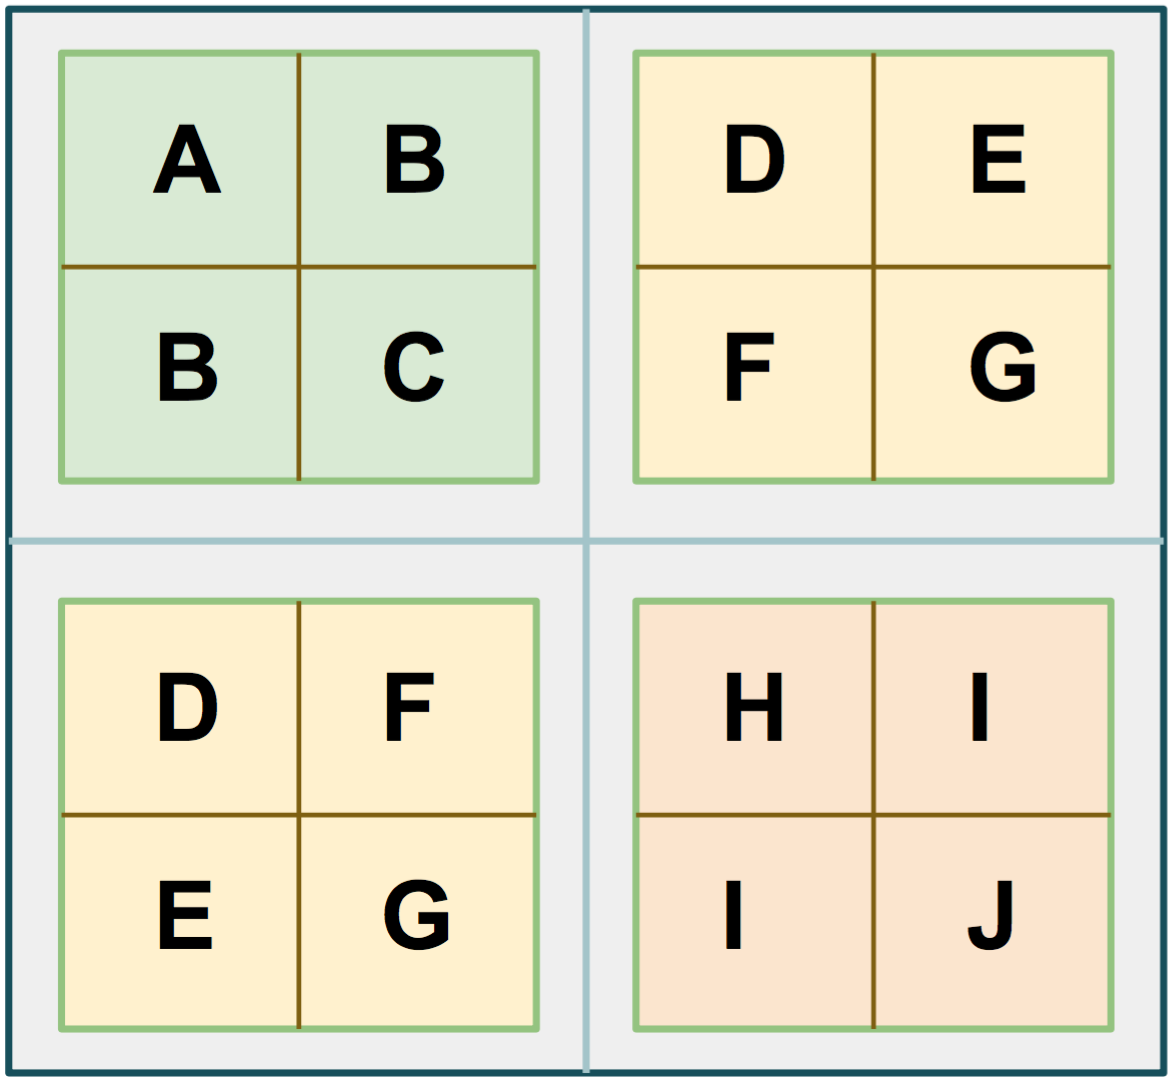
\includegraphics[scale=0.3]{img/mat.png}
  \caption{Loop tiling for $4\times 4$matrix.}
  \label{fig:n}
\end{figure}

In \ref{fig:n} alphabetic letters represents values in each position
of a $N\times N$ matrix. Blocks with the same color will be loaded
into into cache at the same time(symmetrical in X and Y). And the
position with the same letter will switch value. 

The previous paragraph however, will be strongly criticized if this is
an assignment in a CS6+ class since the whole thing is not clear and
it leads to infinite way of understanding even for a native English
speaker. So the process of loop tiling is shown below:
\begin{itemize}
\item Cache was empty at first and the first round will experience a
  missing hit;
\item The tile is gonna be loaded and iterated without new cache
  misses;
\item When operation on the tile is finished, there will be new miss
  hit, and new tile is gonna be loaded again;
\item Same process goes on until program reaches the end.
\end{itemize}

So how much is the new cache misses. When going through this part
before the deadline I actually was not very clear about every
step. And after that I consulted a couple guys about cache
mechanism. 

Let $M$ denote the total cache misses and $b$ the block grid size, in
this case $b=2\times 2=4$

Then we have:
$$M\approx 2\frac{N^2}{b} = \frac{N^2}{2}$$

In a word:
\begin{itemize}
\item No tiling:  $N^2+\frac{N^2}{8}$ 
\item With tiling: $\frac{N^2}{2}$
\end{itemize}

Different methods and algorithms will have different results in for
tiling cache miss. 



\end{document}

%%% Local Variables:
%%% mode: latex
%%% TeX-master: t
%%% End:
